% !TeX spellcheck = da_DK
\section{Samlet systemtest}
Efter de enkelte blokke er blevet testet og godkendt hver for sig, skal det samlede system testes. Formålet med den samlede systemtest er at kontrollere, hvorvidt systemet overholder de overordnede funktionelle krav jævnfør afsnit \ref{FunkKrav}, side \pageref{FunkKrav}. Der anvendes samme fremgangsmåde for test af det samlede system, som af de øvrige blokke; Først simuleres systemet i LTspice, hvorefter det implementeres og testes.

\subsection{Simulering}
I simuleringen af det samlede system kontrolleres det, som i de øvrige simuleringer, om systemet fungerer ideelt. I simuleringen undersøges der, hvorvidt feedbackkomponenterne tænder ved de angivende hældningsgrader. Denne kontrol udføres ved at indsende et sinussignal som inputspænding til systemet, der teoretisk skal tænde hhv. de enkelte LED'er og vibratorer. Simuleringen udføres efter samme principper, som simuleringen af feedbackkonfigurationen, jævnfør afsnit \ref{feedback_simulering}, side \pageref{feedback_simulering}. Designet af det samlede system ses på \figref{fig:samlet_system}:
\begin{figure}[H]
	\centering
	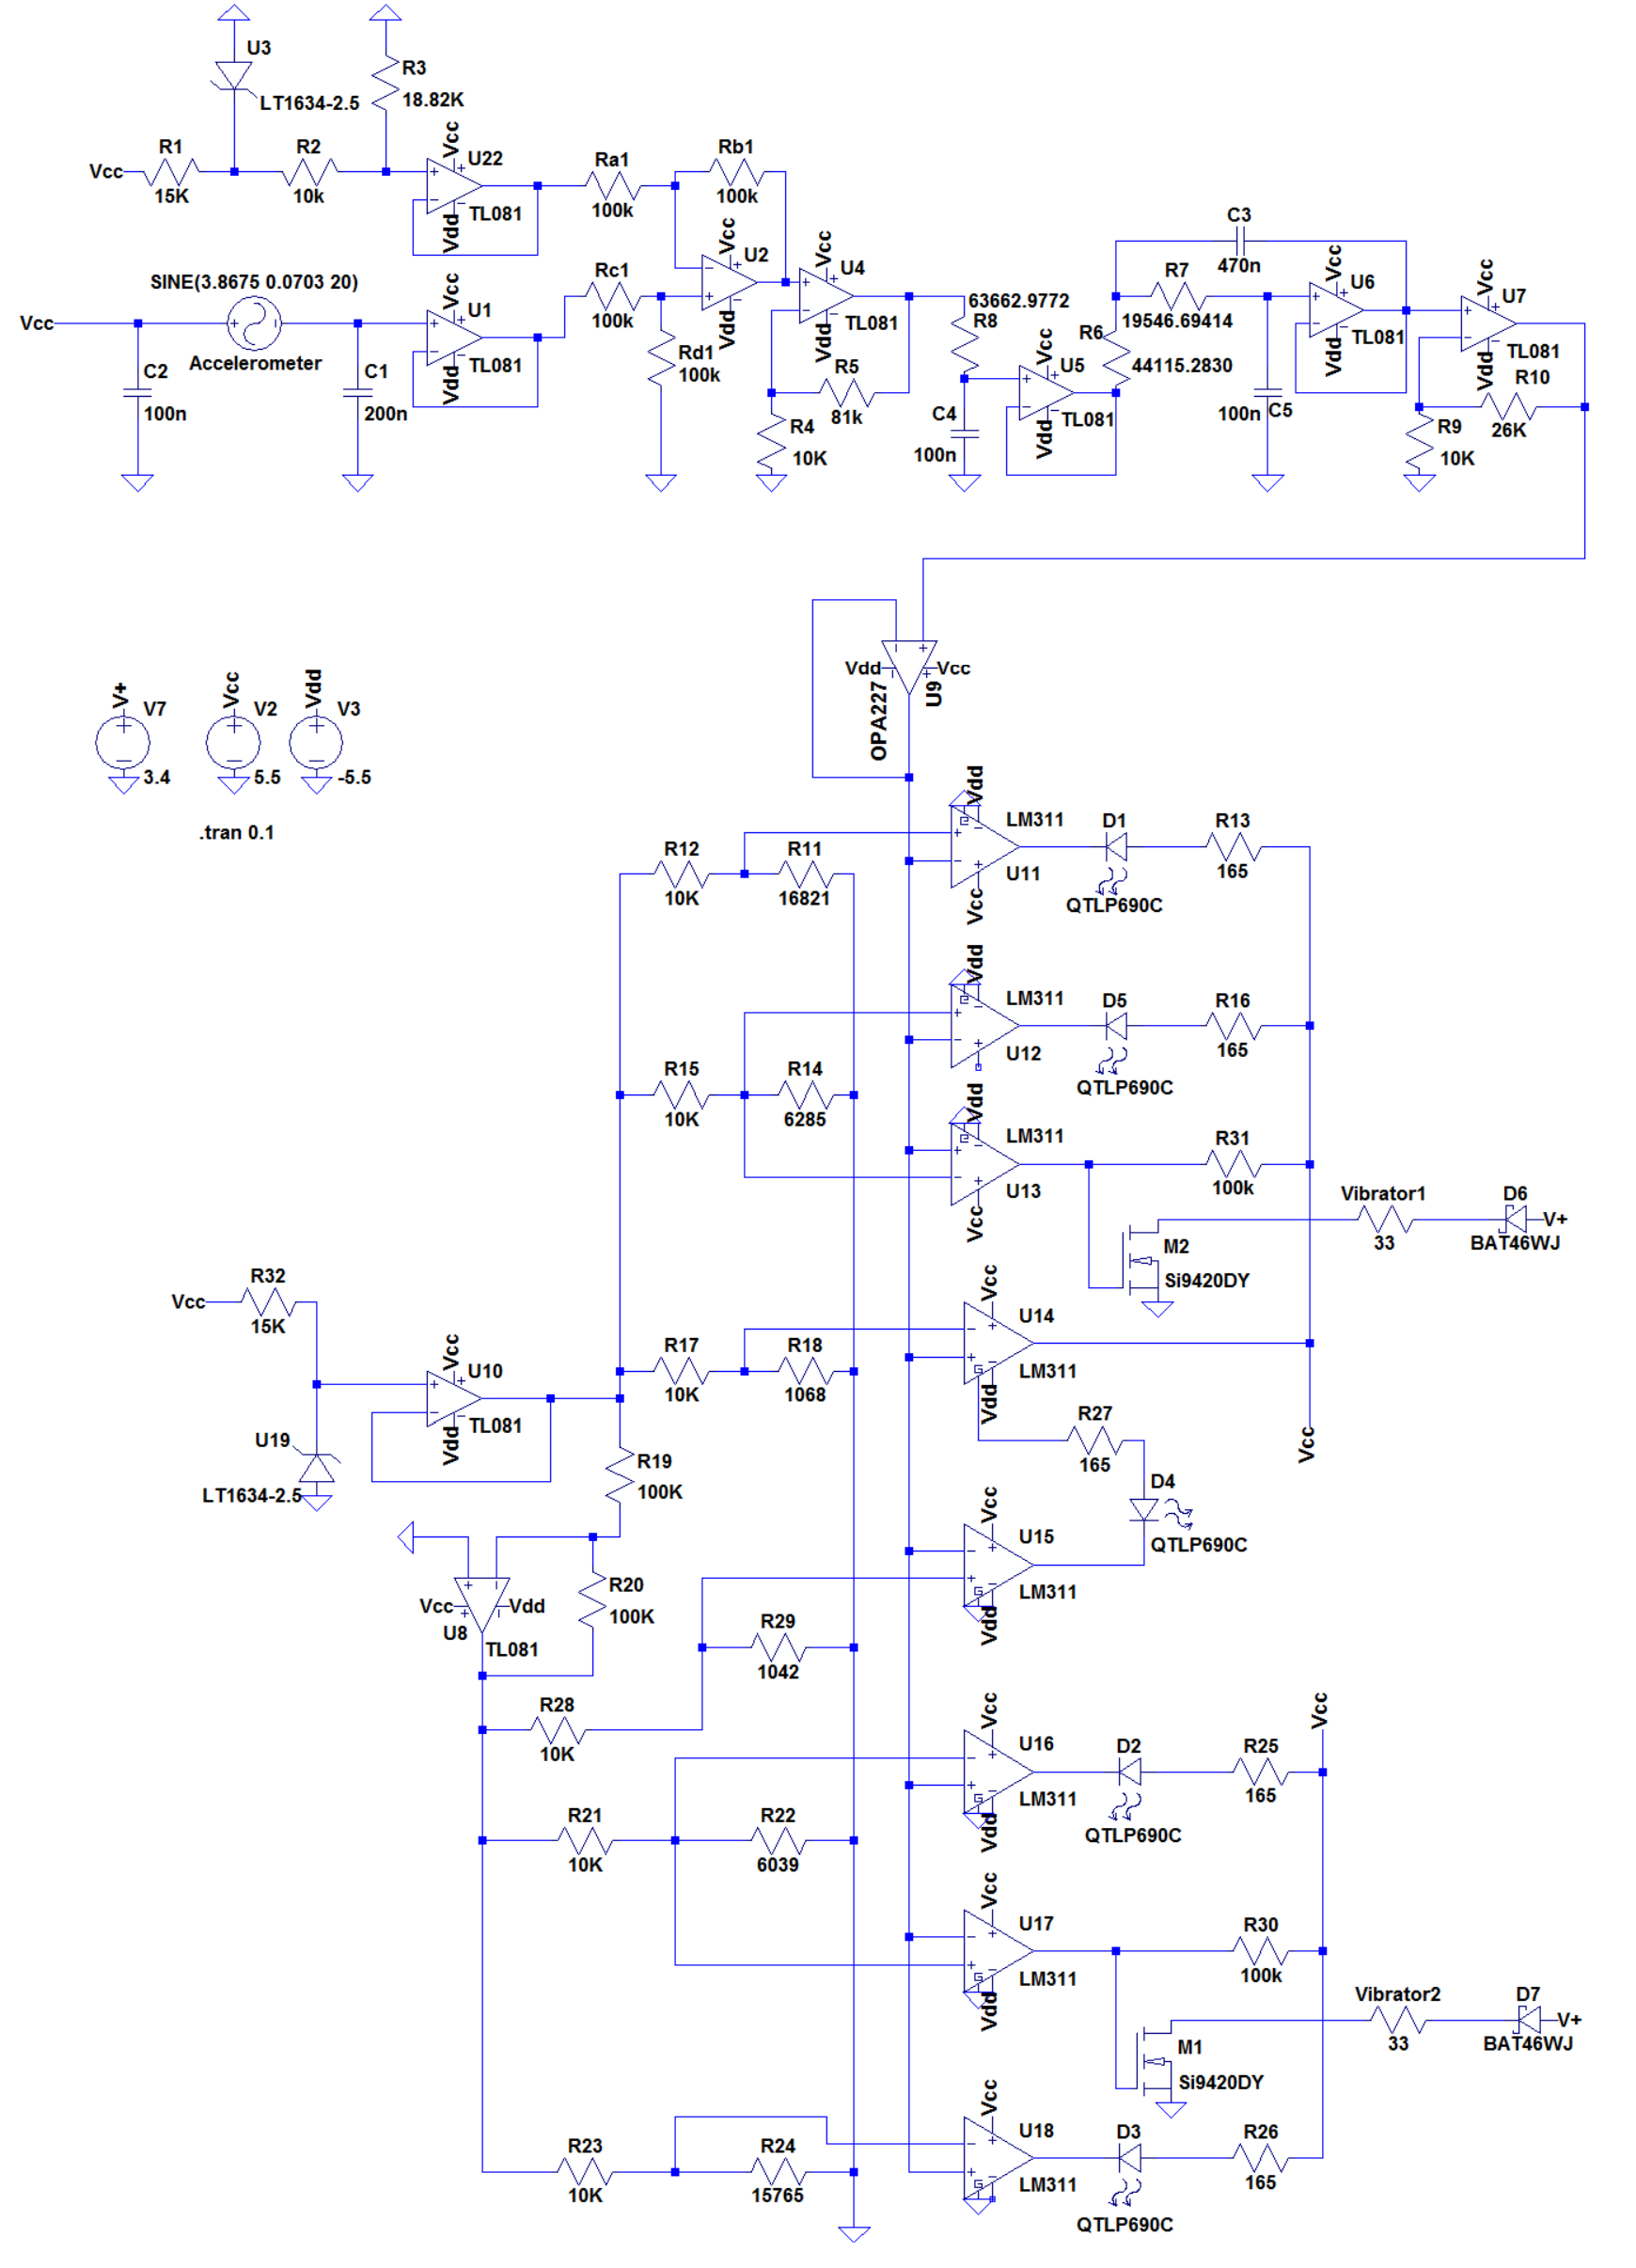
\includegraphics[scale=.4]{figures/cProblemloesning/Samlet_systemUL2.PNG}
	\caption{På figuren ses designet af det samlede system.}
	\label{fig:samlet_system}
\end{figure}
\noindent Sinussignalets amplitude udregnes til at være:
\begin{eqnarray}
0.0037\text{V} \cdot 19^{\circ} = 0.0703V
\end{eqnarray}
\noindent Den maksimale spænding fra accelerometret ved $1^{\circ}$ hældning er $0.0037$V. Dette ganges med $19$, da den røde LED teoretisk tænder ved $13^{\circ}$ og arbejdsområdet for forstærkeren i tilpasningsblokken er $\pm25^{\circ}$. Dermed er midtpunktet mellem disse to grænser $19^{\circ}$. Det kan derved undersøges igennem simuleringen, hvorvidt systemet teoretisk opfylder de overordnede funktionelle krav.\\
Der foretages nogle basale ændringer i det opstillede system i LTspice, som ses \figref{fig:samlet_system}, for at en computer kan køre simuleringen. Ændringerne omfatter, at blokke, som leverer en uændret spænding, udskiftes med spændingsforsyninger. Disse leverer den spændingsværdi, som de giver i simuleringen. Dermed fjernes nogle operationsforstærkere fra det teoretisk opstillede system, hvorefter computeren kan konfigurere simuleringen af det samlede system. Designet med basale ændringer kan ses på \figref{fig:samlet_system}
\begin{figure}[H]
	\centering
	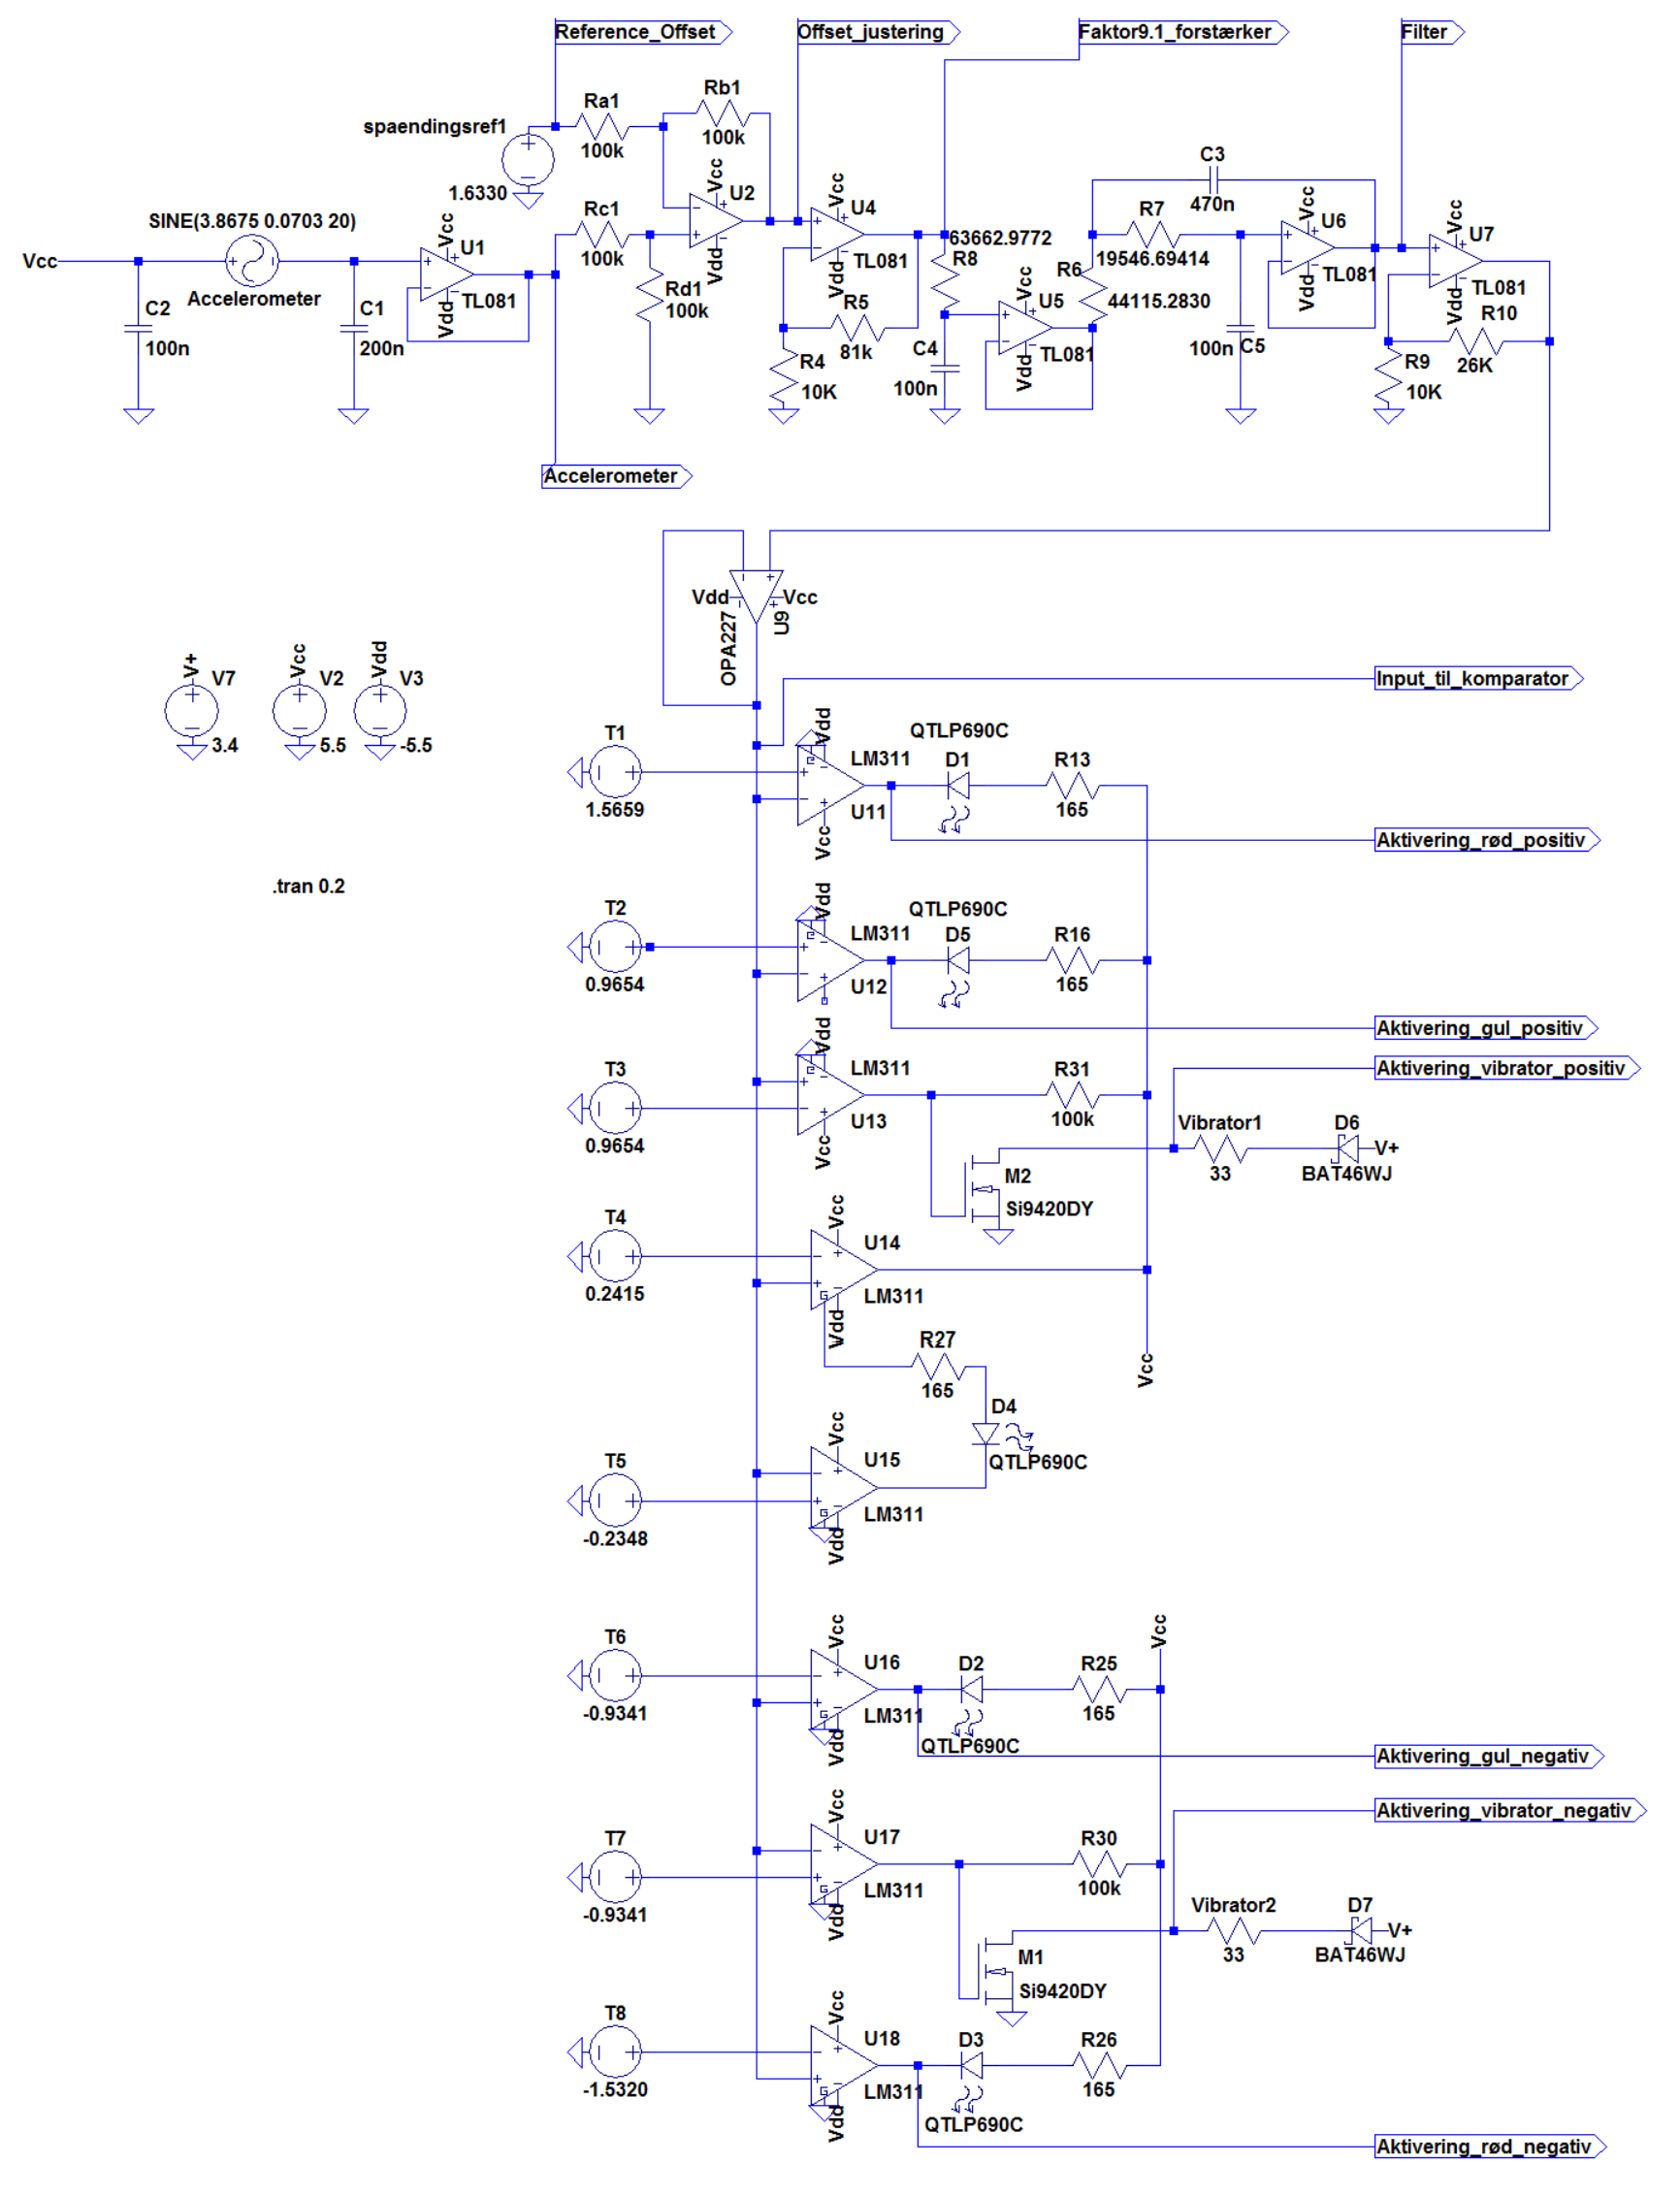
\includegraphics[scale=.42]{figures/cProblemloesning/Samlet_system3_sim.PNG}
	\caption{På figuren ses designet af det forenklede samlede system med labels, der indikerer målepunkterne for de følgende simuleringer. Derved kan blokkenes effekt på signalet følges undervejs i systemet. Referencespændingen til offsetjusteringsblokken er erstattet med en spændingsforsyning på $1.6325$V, hvilket konfigurationen, som før var forbundet her, teroretisk skulle levere. Derudover er hele konfigurationen, som skal tilføre tærskelværdier til komparatorerne, udskiftet med spændingsforsyninger, der leverer den simulerede tærskelværdi til hver komparator, som er målt i \tableref{Tab:test_reference1}, side \pageref{Tab:test_reference1}.}
	\label{fig:samlet_system}
\end{figure}
\noindent Simuleringen kan herefter foretages. Resultatet fra simuleringen ses på nedenstående figurer.
\begin{figure}[H]
	\centering
	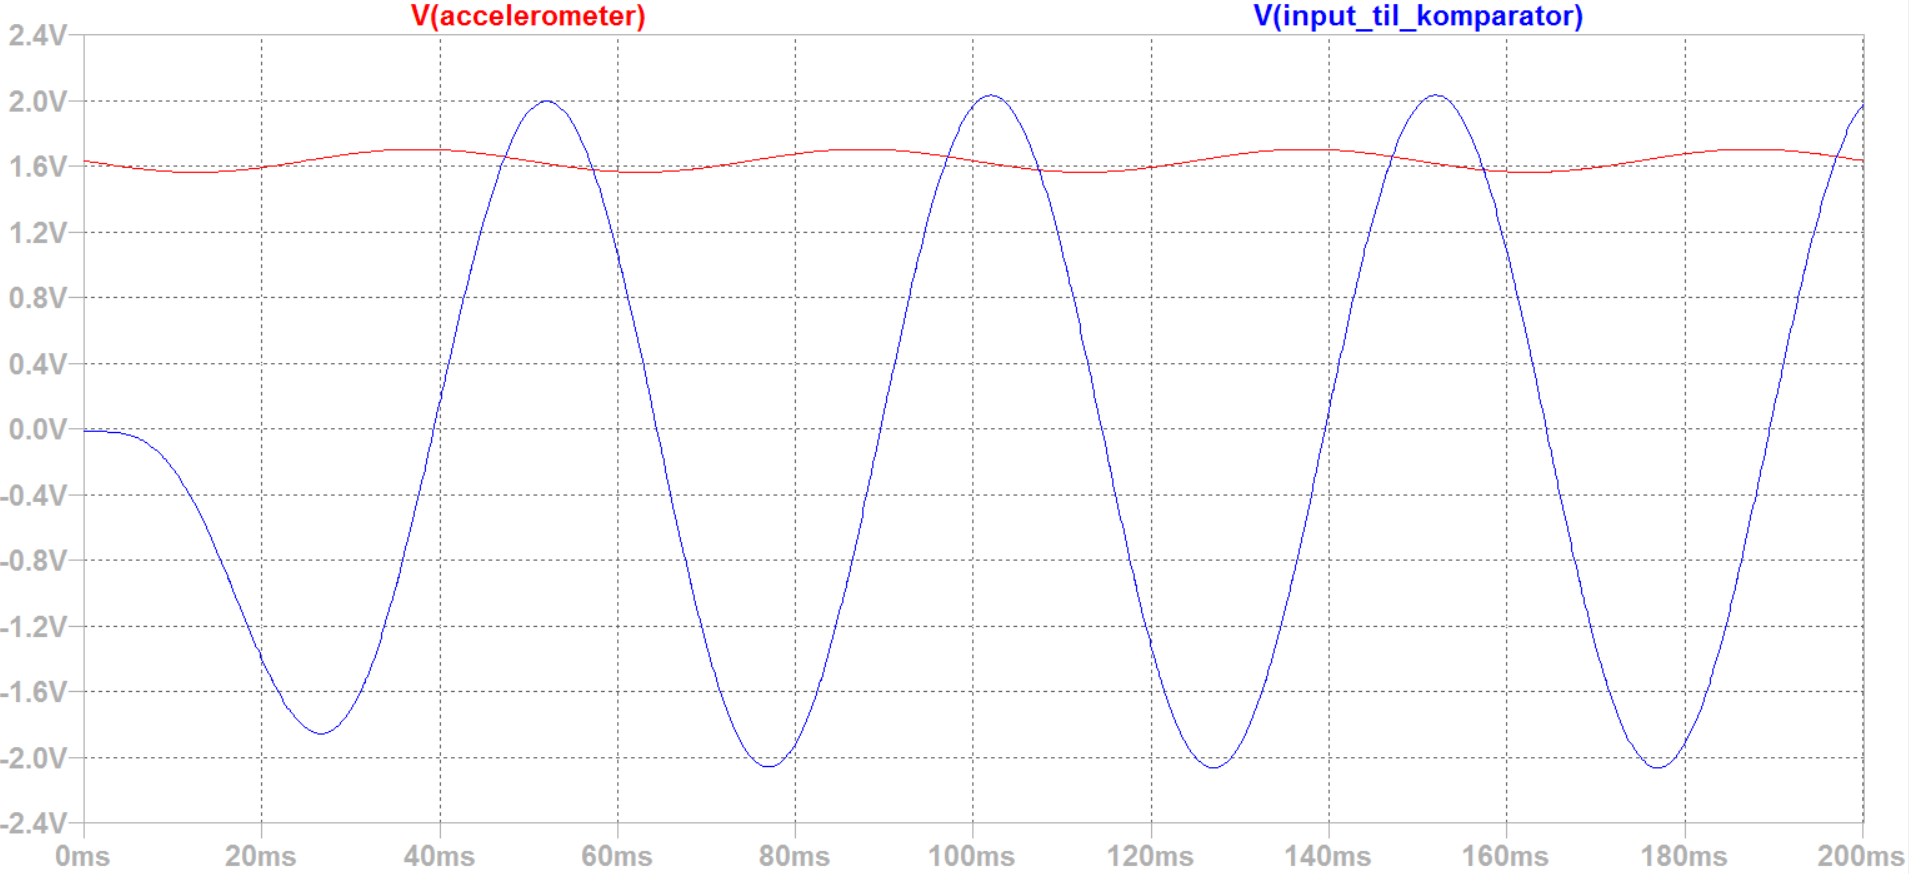
\includegraphics[scale=.38]{figures/cProblemloesning/Samlet_system_sim12.PNG}
	\caption{På figuren ses outputtet fra accelerometret plottet sammen med inputtet til komparatorblokken. Der ses, at signalets offset er blevet justeret, så signalet nu er centreret omkring 0V. Derudover er signalet blevet forstærket to gange og filtreret. Dette ses ved, at amplituden er blevet forstørret og frekvensen er forskudt.}
	\label{fig:samlet_system_sim1}
\end{figure}
\begin{figure}[H]
	\centering
	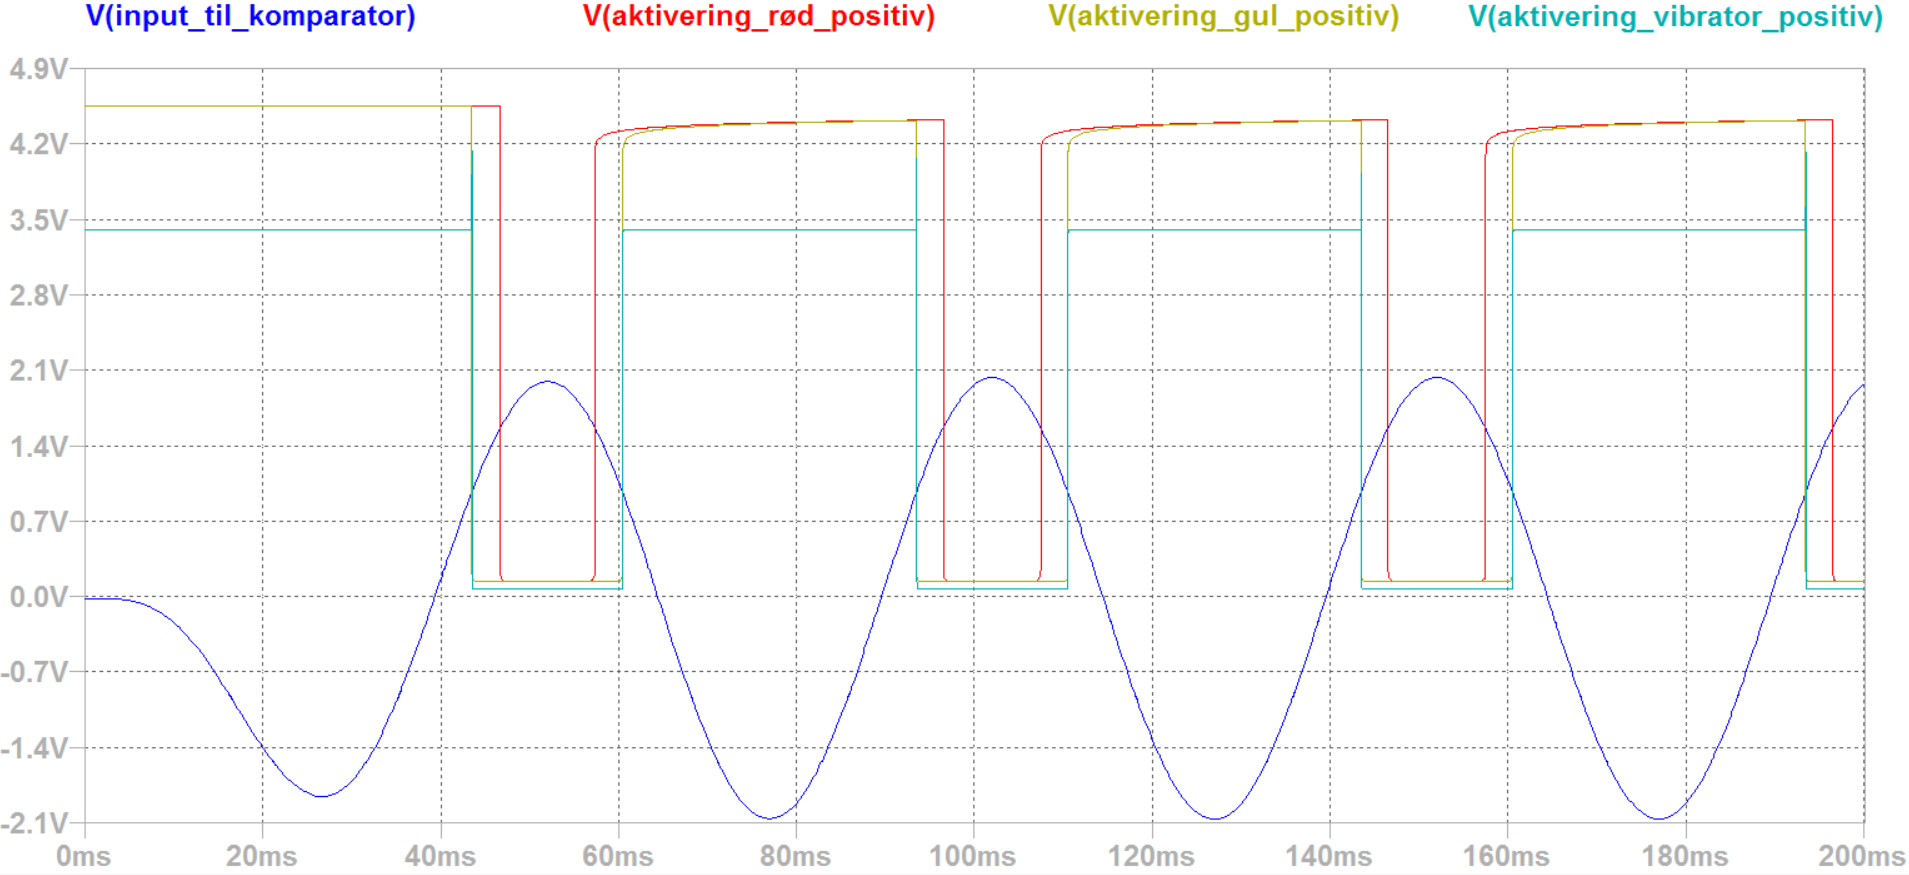
\includegraphics[scale=.38]{figures/cProblemloesning/Samlet_system_sim3.PNG}
	\caption{På figuren ses inputtet til feedbackblokken plottet sammen med visualiseringen af, hvornår LED'erne samt vibratorerne i positiv retning tændes. På figuren aflæses det, at den røde LED tændes, når inputsignalet er over ca. $1.5$V. Den gule LED samt vibratoren i positiv retning tænder, når inputsignalet er ca. $0.9$V.}
	\label{fig:samlet_system_sim2}
\end{figure}
\begin{figure}[H]
	\centering
	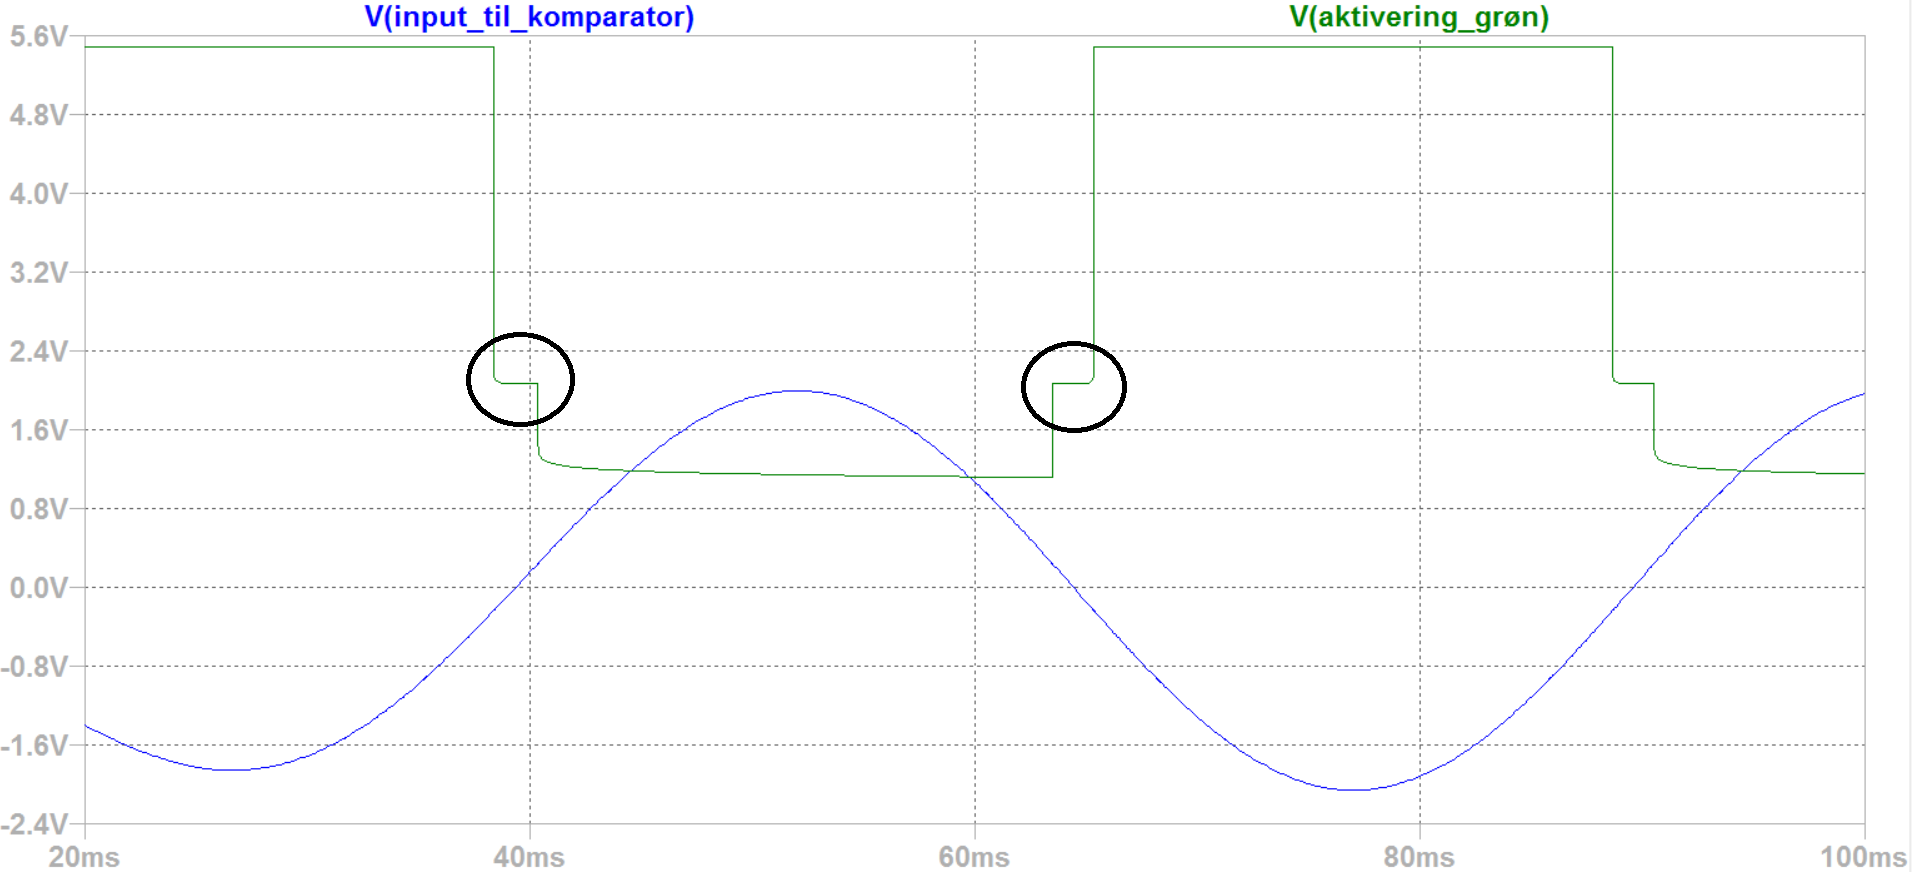
\includegraphics[scale=.38]{figures/cProblemloesning/Samlet_system_sim5.PNG}
	\caption{På figuren ses inputtet til komparatorblokken plottet sammen med visualiseringen af, hvornår den grønne LED er tændt. På figuren aflæses det, at den grønne LED er designet i en vindues-komparatorkonfiguration, hvilket betyder, at den kun er aktiv i hakket, som er markeret med to sorte cirkler på figuren. Det fremgår, at den er aktiv mellem -$0.2$V og $0.2$V.}
	\label{fig:samlet_system_sim5}
\end{figure}
\begin{figure}[H]
	\centering
	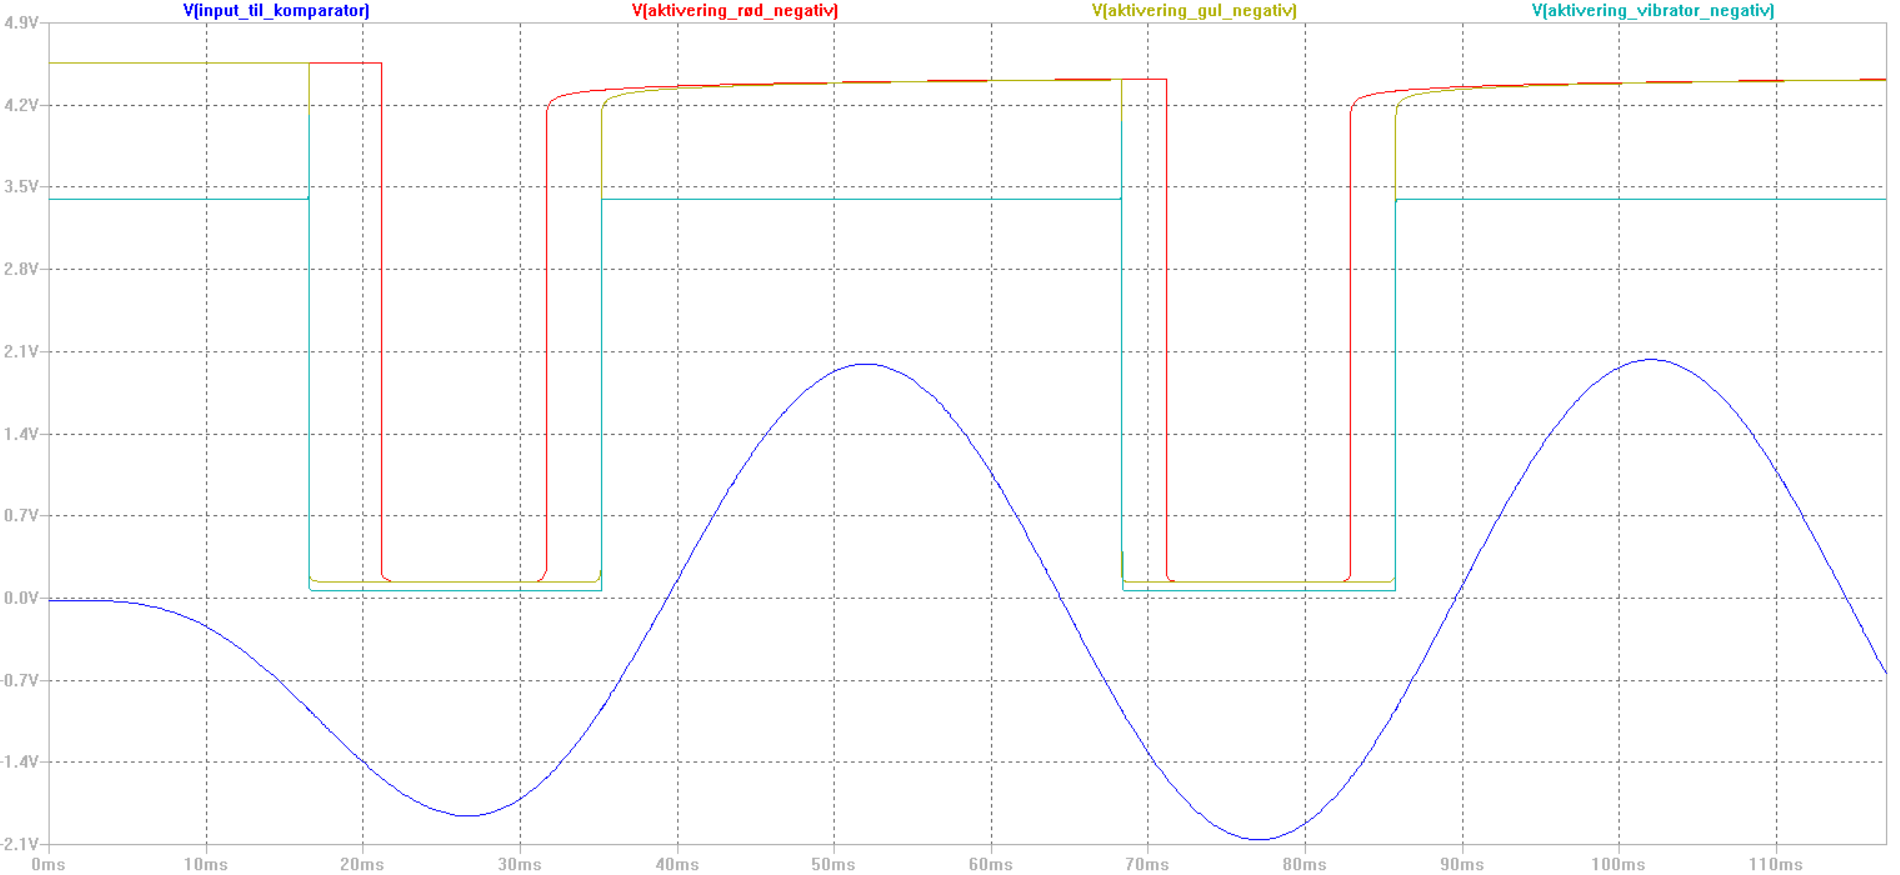
\includegraphics[scale=.38]{figures/cProblemloesning/Samlet_system_sim4.PNG}
	\caption{På figuren ses inputtet til komparatorblokken plottet sammen med visualiseringen af, hvornår LED'erne samt vibratorerne i negativ retning tændes. På figuren aflæses det, at den røde LED tændes, når inputsignalet er over ca. -$1.5$V. Den gule LED samt vibratoren tændes, når inputsignalet er ca. -$0.9$V.}
	\label{fig:samlet_system_sim3}
\end{figure}
\noindent På baggrund af de fortagede aflæsninger vurderes det, at LED'erne samt vibratorerne tændes ved de korrekte tærskelværdier. Accelerometerets output aflæses ved aktivering af de enkelte feedbackkomponenter. Dette ses i \tableref{tab:samlet_sim}:
\begin{table}[H]
	\centering
	\begin{tabular}{l|l|l|l|}
		\cline{2-4}
		\textit{}                                                                                              & \textit{\begin{tabular}[c]{@{}l@{}}Output fra\\ accelerometer\end{tabular}} & \textit{\begin{tabular}[c]{@{}l@{}}Graders\\ hældning\end{tabular}}          & \textit{Afvigelse}                                      \\ \hline
		\multicolumn{1}{|l|}{\textit{\begin{tabular}[c]{@{}l@{}}Rød LED\\ positiv\end{tabular}}}               & $1.6763$V                                                                   & $11.84^{\circ}$                                                              & $8.92\%$                                                   \\ \hline
		\multicolumn{1}{|l|}{\textit{\begin{tabular}[c]{@{}l@{}}Gul LED\\og vibrator\\ positiv\end{tabular}}} & $1.6620$V                                                                   & $7.97^{\circ}$                                                               & $0.38\%$                                                   \\ \hline
		\multicolumn{1}{|l|}{\textit{Grøn LED}}                                                                & \begin{tabular}[c]{@{}l@{}}$1.6400$V\\ $1.6251$V\end{tabular}               & \begin{tabular}[c]{@{}l@{}}$2.03^{\circ}$ til\\ -$2.06^{\circ}$\end{tabular} & \begin{tabular}[c]{@{}l@{}}$1.5\%$\\ $3\%$\end{tabular} \\ \hline
		\multicolumn{1}{|l|}{\textit{\begin{tabular}[c]{@{}l@{}}Gul LED\\og vibrator\\ negativ\end{tabular}}} & $1.6027$V                                                                   & -$8.27^{\circ}$                                                              & $3.4\%$                                                    \\ \hline
		\multicolumn{1}{|l|}{\textit{\begin{tabular}[c]{@{}l@{}}Rød LED\\ negativ\end{tabular}}}               & $1.5843$V                                                                   & -$13.38^{\circ}$                                                              & $2.9\%$                                                    \\ \hline
	\end{tabular}
	\caption{I tabellen ses resultatet af det simulerede samlede system ved aktivering af de enkelte feedbackkomponenter og den procentvise afvigelse fra de definerede hældningsgrader.}
	\label{tab:samlet_sim}
\end{table}


\subsection{Implementering og test}\label{samlet_systemtest_ref}
Det samlede system implementeres på to breadboards. Opsætningen kan ses på \figref{fig:samlet_system_real}
\begin{figure}[H]
	\centering
	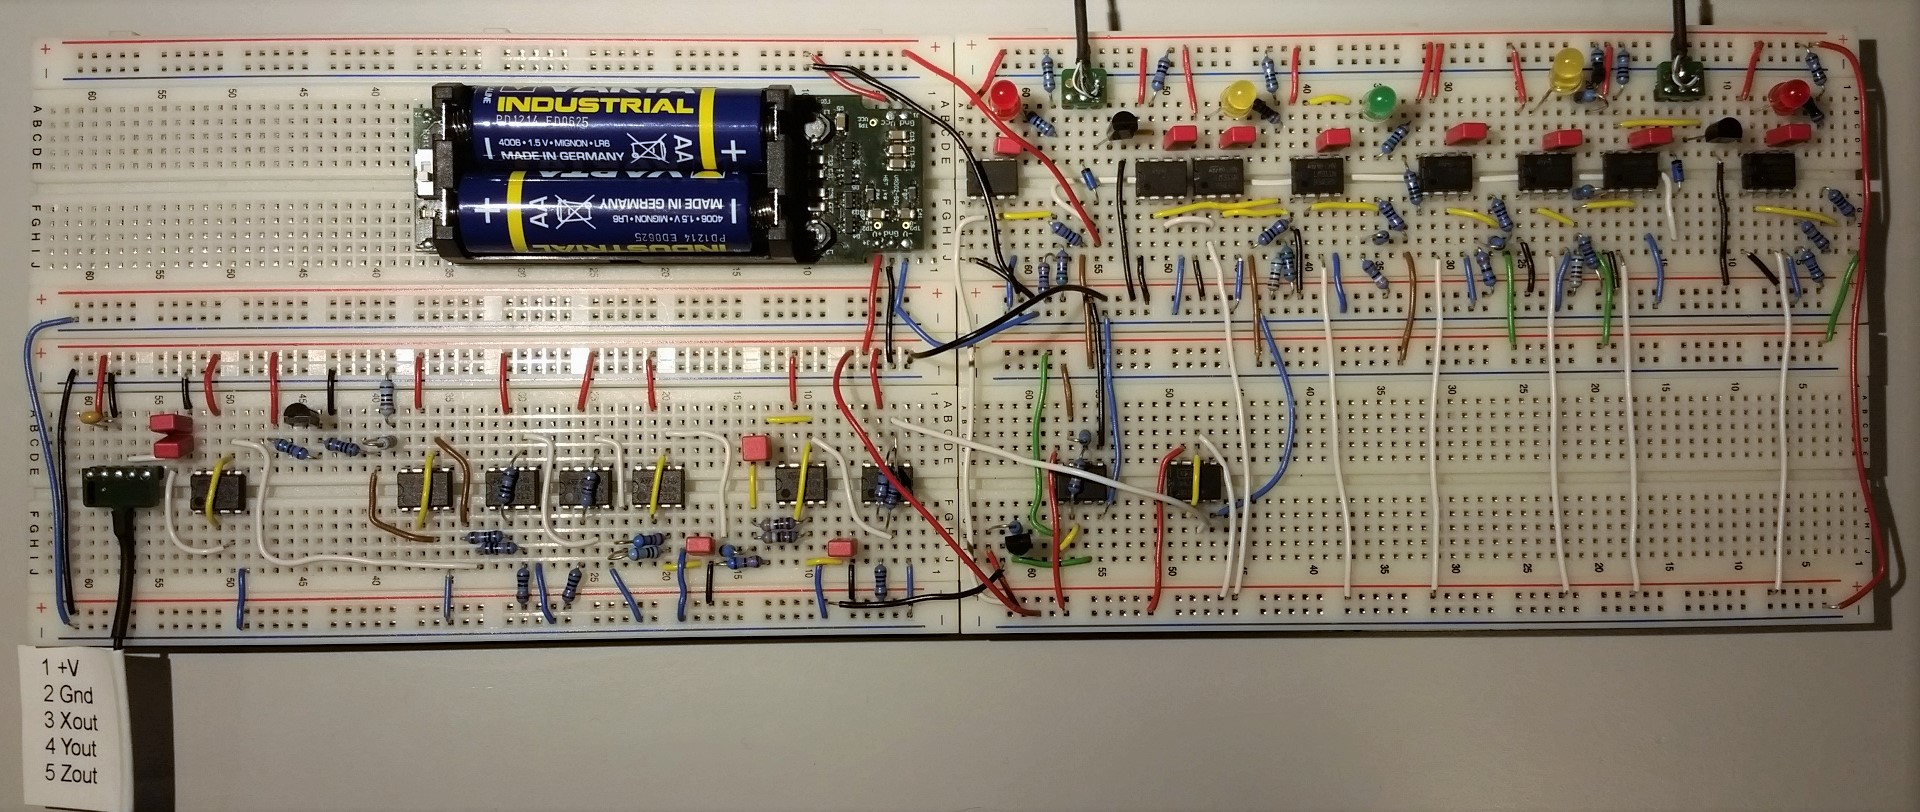
\includegraphics[scale=.22]{figures/cProblemloesning/Samlet_system2.jpg}
	\caption{På figuren ses implementeringen af systemet. Ledningernes farve angiver forskellige funktioner: De hvide leder signalet fra accelerometret igennem systemet og de røde og blå leder hhv. den positive og negative spændingsforsyning til de forskellige komponenter i systemet. De sorte ledninger leder til ground, og de gule ledninger fungerer som forbindelsesveje. De grønne og brune ledninger leder hhv. en positiv og negativ referencespænding til offsettet og komparatorerne.}
	\label{fig:samlet_system_real}
\end{figure}
\noindent Herefter kan det samlede system blive testet. Systemtesten deles op i to - først en test af det analoge output og efterfølgende en test af det digitale output. \\
\noindent Det måles, hvorvidt systemet opfylder de overordnede funktionelle krav jævnfør afsnit \ref{FunkKrav}, side \pageref{FunkKrav}, ved at hælde accelerometeret i positiv og negativ retning indtil udløst feedback og ved disse tidspunkter aflæses outputtet fra accelerometeret på et multimeter. Med udløst feedback menes der, at de enkelte LED'er lyser og vibratorerne vibrerer.
\subsubsection{Test 1}
Ved test af den analoge del af systemet måles spændingsfaldet over LED'erne og vibratorerne før og efter aktivering. Dette gøres ved, at måle spændingen ved katoden og anoden på de enkelte LED'er, når disse er inaktive. Herved fås spændingsfaldet før udløst feedback. Det samme gøres, når LED'erne er aktive. Herved fås spændingsfaldet efter udløst feedback. Samme principper gentages for måling af spændingsfaldet over vibratorerne. Derudover måles outputtet fra accelerometret lige ved udløst feedback. Testen er udformet således for at dokumentere aktiveringen af feedbackmekanismerne. Disse målinger foretages med et multimeter. Resultatet fremgår af \tableref{Tab:resultat:test1a}:
\begin{table}[H]
	\centering
	\begin{tabular}{l|l|l|l|}
		\cline{2-4}
		\textit{}                                                                                 & \textit{\begin{tabular}[c]{@{}l@{}}Spændingsfald over \\ komponent før\\ udløst feedback\end{tabular}} & \textit{\begin{tabular}[c]{@{}l@{}}Output fra\\ accelerometer\\ ved udløst feedback\end{tabular}} & \textit{\begin{tabular}[c]{@{}l@{}}Spændingsfald over\\ komponent efter \\ udløst feedback\end{tabular}} \\ \hline
		\multicolumn{1}{|l|}{\textit{\begin{tabular}[c]{@{}l@{}}Rød LED\\ positiv\end{tabular}}}  & $1.3311$V                                                                                         & $1.6740$V                                                                                    & $2.0605$V                                                                                           \\ \hline
		\multicolumn{1}{|l|}{\textit{\begin{tabular}[c]{@{}l@{}}Vibrator\\ positiv\end{tabular}}} & $0.1$mV                                                                                           & $1.6562$V                                                                                    & $3.1029$V                                                                                           \\ \hline
		\multicolumn{1}{|l|}{\textit{\begin{tabular}[c]{@{}l@{}}Gul LED\\ positiv\end{tabular}}}  & $1.4247$V                                                                                         & $1.6562$V                                                                                    & $2.1187$V                                                                                           \\ \hline
		\multicolumn{1}{|l|}{\multirow{2}{*}{\textit{Grøn LED}}}                                  & \multirow{2}{*}{$1.4611$V}                                                                        &       $1.6377$V                                                                              & \multirow{2}{*}{$2.0196$V}                                                                          \\ \cline{3-3}
		\multicolumn{1}{|l|}{}                                                                    &                                                                                                   & $1.6243$V                                                                                   &                                                                                                     \\ \hline
		\multicolumn{1}{|l|}{\textit{\begin{tabular}[c]{@{}l@{}}Gul LED\\ negativ\end{tabular}}}  & $1.4310$V                                                                                         & $1.6005$V                                                                                    & $2.0700$V                                                                                           \\ \hline
		\multicolumn{1}{|l|}{\textit{\begin{tabular}[c]{@{}l@{}}Vibrator\\ negativ\end{tabular}}} & $0.6$mV                                                                                           & $1.6005$V                                                                                    & $2.9995$V                                                                                           \\ \hline
		\multicolumn{1}{|l|}{\textit{\begin{tabular}[c]{@{}l@{}}Rød LED\\ negativ\end{tabular}}}  & $1.3296$V                                                                                         & $1.5822$V                                                                                    & $2.0324$V                                                                                           \\ \hline
	\end{tabular}
	\caption{I tabellen ses resultatet fra målingerne af den analoge del af systemet.}
	\label{Tab:resultat:test1a}
\end{table}
\noindent Der ses i \tableref{Tab:resultat:test1a}, at der forekommer et spændingsfald over LED'erne, selvom de ikke afgiver synligt lys. Dette skyldes, at der kan løbe en lækstrøm igennem dem, men denne er ikke tilstrækkelig for aktivering af synligt lys. På \figref{fig:samlet_system_LED} ses graferne for forholdet imellem spændingsfaldet over LED'erne og strømmen, der løber igennem, for de enkelte LED'er. \cite{kingbright}
\begin{figure}[H]
	\centering
	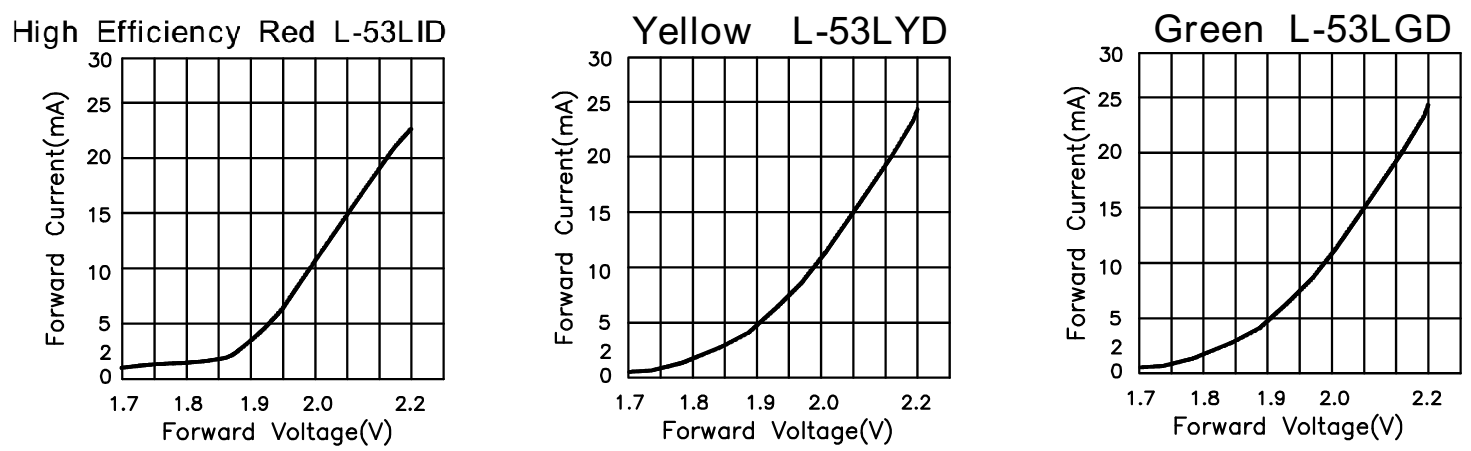
\includegraphics[scale=.45]{figures/cProblemloesning/Samlet_system_LED.PNG}
	\caption{På figuren ses der tre grafer for hhv. den røde, gule og grønne LED. Graferne viser forholdet imellem spændingsfaldet over LED'erne og strømmen, der løber igennem, for de enkelte LED'er. \textit{(Revideret)} \cite{kingbright}}
	\label{fig:samlet_system_LED}
\end{figure}
\noindent Da der ikke er et lineært forhold imellem spændingsfaldet og strømmen på \figref{fig:samlet_system_LED}, er det ikke muligt at vurdere, om LED'erne faktisk er aktiverede ved målingerne i kolonnen i \tableref{Tab:resultat:test1a}, der måler spændingsfaldet over komponenten før udløst feedback. Ifølge databladet for LED'erne vil de aktiveres ved $0.8$mA \cite{kingbright}. Jævnfør afsnit \ref{Afs_Komparator}, side \pageref{Afs_Komparator} vurderes det, at en LED skal modtage $20$mA for at afgive tydeligt lys. Da feedbackblokken er tilpasset til, at denne strøm skal løbe over LED'erne, kan det forventede spændingsfald aflæses på grafernes x-akse for de enkelte LED'er på \figref{fig:samlet_system_LED}. Ud fra disse værdier beregnes afvigelsen for de målte spændingsfald. \\
I fjerde kolonne på \tableref{Tab:resultat:test1a} ses det målte spændingsfald, når der teoretisk løber $20$mA over LED'en. De beregnede afvigelser ses i \tableref{tab:samlet_procent1a}. De teoretiske værdier for spændingsfaldet er aflæst på x-aksen ud fra $20$mA på y-aksen på \figref{fig:samlet_system_LED}.
\begin{table}[H]
	\centering
	\begin{tabular}{l|l|l|l|}
		\cline{2-4}
		\textit{} & \textit{\begin{tabular}[c]{@{}l@{}}Teoretisk\\ spændingsfald\end{tabular}} & \textit{\begin{tabular}[c]{@{}l@{}}Målte\\ spændingsfald\end{tabular}} & \textit{Afvigelse} \\ \hline
		\multicolumn{1}{|l|}{\textit{\begin{tabular}[c]{@{}l@{}}Rød LED\\ positiv\end{tabular}}} & $2.14$V                                                                    & $2.0605$V                                                              & $3.71\%$              \\ \hline
		\multicolumn{1}{|l|}{\textit{\begin{tabular}[c]{@{}l@{}}Gul LED\\ positiv\end{tabular}}} & $2.15$V                                                                    & $2.1187$V                                                              & $1.46\%$              \\ \hline
		\multicolumn{1}{|l|}{\textit{Grøn LED}}                                                  & $2.14$V                                                                    & $2.0196$V                                                              & $5.63\%$              \\ \hline
		\multicolumn{1}{|l|}{\textit{\begin{tabular}[c]{@{}l@{}}Gul LED\\ negativ\end{tabular}}} & $2.15$V                                                                    & $2.0700$V                                                              & $3.73\%$              \\ \hline
		\multicolumn{1}{|l|}{\textit{\begin{tabular}[c]{@{}l@{}}Rød LED\\ negativ\end{tabular}}} & $2.14$V                                                                    & $2.0324$V                                                              & $5.03\%$              \\ \hline
	\end{tabular}
	\caption{I tabellen ses afvigelsen fra det forventede spændingsfald ved aktivering af LED'erne.}
	\label{tab:samlet_procent1a}
\end{table}
\noindent Det fremgår af \tableref{tab:samlet_procent1a}, at der er afvigelser imellem det målte og det forventede spændingsfald for alle LED'erne. Alle de målte værdier ligger under de teoretiske værdier, hvorfor det må antages, at LED'ernes lys er svagere. Da det typiske interval for spændingsfaldet ved synligt lys ligger på $1.7$-$1.9$V og maksimalt på $2.0$-$2.2$V jævnfør afsnit \ref{Afs_Komparator} på side \pageref{Afs_Komparator}, vurderes det imidlertid, at LED'erne udløser deres feedback, og at det sker efter hensigten.\\
Vibratorerne aktiveres, når der sker et spændingsfald over dem på $2.3$V \cite{Machinery2009}. Teoretisk bør der ikke forekomme spændingsfald over vibratorerne, når disse er slukkede. Ud fra målingerne i \tableref{Tab:resultat:test1a} vurderes det, at dette er gældende, da der arbejdes med reelle komponenter under implementeringen. Ved udløst feedback sker der et spændingsfald for begge vibratorer på ca. $3$V. Dermed er spændingsfaldet over grænsen for aktivering, og det vurderes derfor, at vibratorerne udløser deres feedback, og at det sker efter hensigten. \\
Ud fra de målte outputværdier fra accelerometeret kan det beregnes, om feedbackmekanismerne aktiveres ved de definerede hældningsgrader jævnfør afsnit \ref{KomparatorAfs}, side \pageref{KomparatorAfs}. Dette gøres ved at tage outputværdien, trække offsettet i accelerometret fra og derefter dividere dette med hhv. -$0.0036$V og $0.0037$V for output i negativ og positiv retning. \\
\begin{equation}\label{eq:graderLED_2}
\dfrac{(1.6740 - 1.6325)}{0.0037} = 11.22^{\circ}\text{ for aktivering af rød LED i positiv retning}
\end{equation}
\begin{equation}
\dfrac{(1.6562 - 1.6325)}{0.0037} = 6.41^{\circ}\text{ for aktivering af gul LED samt vibrator i positiv retning}
\end{equation}
\begin{equation}
\dfrac{(1.6377 - 1.6325)}{0.0037} = 1.41^{\circ}\text{ for deaktivering af grøn LED i positiv retning}
\end{equation}
\begin{equation}
\dfrac{(1.6243 - 1.6325)}{-0.0036} = 2.28^{\circ}\text{ for deaktivering af grøn LED i negativ retning}
\end{equation}
\begin{equation}
\dfrac{(1.6005 - 1.6325)}{-0.0036} = 8.89^{\circ}\text{ for aktivering af gul LED samt vibrator i negativ retning}
\end{equation} 
\begin{equation}\label{eq:graderLED_1}
\dfrac{(1.5822 - 1.6325)}{-0.0036} = 13.97^{\circ}\text{ for aktivering af rød LED i negativ retning}
\end{equation}
\noindent I overstående ligninger ses en afvigelse i accelerometerets hældning ift. de definerede grader for aktivering af feedbacken. Grunden til dette kan være, at referencespændingen til offsettet måles til $1.6302$V, hvilket er -$0.0023$V fra det teoretiske offset i accelerometret. Derved forskydes offsettet mod de negative spændingsværdier, og graderne for hældning af accelerometret i negativ retning vil blive større, mens graderne vil blive mindre i positiv retning. Derudover skal der tages højde for afvigelserne i de enkelte blokke i systemet, som undervejs er blevet tolereret og accepteret. Disse vil tilsammen kunne skabe en større afvigelse for det samlede system. \\
Ved rotation af accelerometret observeres det, at systemet fungerer ift. de overordnede krav, da accelerometret roteres indtil udløst feedback. Det observeres, at feedbacken udløses i den forventede rækkefølge.\\
På baggrund af målingerne og de vurderede fejlkilder godkendes den analoge del af systemet og det vurderes, at det virker efter hensigten ift. de overordnede funktionelle krav.\\

%%%%%%%%%%%%%%%%%%%%%%%%%%%%%%%%%%%5
Der ses af testen afvigelser for samtlige grader, hvor LED'erne samt vibratorerne aktiveres ift. de definerede grader. Der ses i \eqref{eq:graderLED_1}-\ref{eq:graderLED_2} på side \pageref{eq:graderLED_1}, at den maksimale afvigelse i grader er $13^{\circ} - 11.22^{\circ} = 1.78^{\circ}$, hvilket svarer til $13.69\%$. Der forekommer således en højere procentvis afvigelse i denne test sammenlignet med de udregnede afvigelser for test af de enkelte blokke. Det vurderes, at denne afvigelse altså kan forventes grundet afvigelser i de enkelte blokke. Hvis der f.eks. tages udgangspunkt i outputtet fra accelerometret ved aktivering af de enkelte LEDer og vibratorer, kan afvigelsen for de enkelte signaler beregnes, hvis der tages højde for kalibrering af offsettet. Dette ses i \tableref{tab:nye_afv}.

\begin{table}[H]
	\centering
	\begin{tabular}{l|l|l|l|l|}
		\cline{2-5}
		\textit{}                                                                                              & \textit{\begin{tabular}[c]{@{}l@{}}Output fra\\ accelerometer\end{tabular}} & \textit{\begin{tabular}[c]{@{}l@{}}Output uden\\ offset\end{tabular}} & \textit{\begin{tabular}[c]{@{}l@{}}Graders\\ hældning\end{tabular}}          & \textit{Afvigelse}                                      \\ \hline
		\multicolumn{1}{|l|}{\textit{\begin{tabular}[c]{@{}l@{}}Rød LED\\ positiv\end{tabular}}}               & $1.6740$V                      &       $0.0438$V                                        & $11.84^{\circ}$                                                              & $8.92\%$                                                   \\ \hline
		\multicolumn{1}{|l|}{\textit{\begin{tabular}[c]{@{}l@{}}Gul LED\\og vibrator\\ positiv\end{tabular}}} & $1.6562$V            &             $0.026$V                                             & $7.03^{\circ}$                                                               & $12.13\%$                                                   \\ \hline
		\multicolumn{1}{|l|}{\textit{Grøn LED}}                                                                & \begin{tabular}[c]{@{}l@{}}$1.6377$V\\ $1.6243$V\end{tabular}   &  \begin{tabular}[c]{@{}l@{}}$0.0075$V\\ -$0.0059$V\end{tabular}            & \begin{tabular}[c]{@{}l@{}}$2.03^{\circ}$ til\\ -$1.64^{\circ}$\end{tabular} & \begin{tabular}[c]{@{}l@{}}$1.5\%$\\ $18\%$\end{tabular} \\ \hline
		\multicolumn{1}{|l|}{\textit{\begin{tabular}[c]{@{}l@{}}Gul LED\\og vibrator\\ negativ\end{tabular}}} & $1.6005$V            & -$0.0297$V                                                       & -$8.25^{\circ}$                                                              & $3.13\%$                                                    \\ \hline
		\multicolumn{1}{|l|}{\textit{\begin{tabular}[c]{@{}l@{}}Rød LED\\ negativ\end{tabular}}}               & $1.5822$V              & -$0.0480$V                                                     & -$13.33^{\circ}$                                                              & $2.56\%$                                                    \\ \hline
	\end{tabular}
	\caption{I tabellen ses, at hvorledes de enkelte hældningsgrader ændres, hvis der tages højde for afvigelsen i referencespændingen til offsetjusteringsblokken.}
	\label{tab:nye_afv}
\end{table}

%\begin{eqnarray}
%1.6740 - 1.6302 = 0.0438 \\
%\dfrac{0.0438}{0.0037} = 11.84^{\circ}
%\end{eqnarray}
Der ses i tabellen, at LED'erne aktiveres ved en anden hældningsgrad, hvis der tages højde for kalibrering af offsettet. Generelt ses en lavere afvigelse ift. den forventede og målte hældningsgrad for hvornår feedbacken skal udløses. For den grønne LED ses en større afvigelse i negativ retning på $18$\% ved en hældningsgrad på $1.64^{\circ}$. Flere af de benyttede komponenter har et indbygget offset, som f.eks. operationsforstærkere, hvormed dette også kan påvirke både de enkelte blokke og det samlede system. Der forventes ikke, at afvigelsen for det samlede system vil forsvinde helt, selvom der tages højde for blokkenes individuelle afvigelse, da der også skal medregnes eventuelle fejl ved målemetoderne ift. aflæsning eller upræcist udstyr. \\
%%%%%%%%%%%%%%%%%%%%%%%%%%%%%%%%%%%%%%%%%%%

\subsubsection{Test 2}
Ved test af den digitale del af systemet undersøges det, hvorvidt systemet kan give et digitalt output, som kan aflæses realtime og gemmes som en billedfil jævnfør de overordnede funktionelle krav i afsnit \ref{FunkKrav}, side \pageref{FunkKrav}. \\
Ved testen roteres accelerometret tilfældigt i positiv og negativ retning, hvilket er afbilledet på \figref{fig:samlet_system_digital}:
\begin{figure}[H]
	\centering
	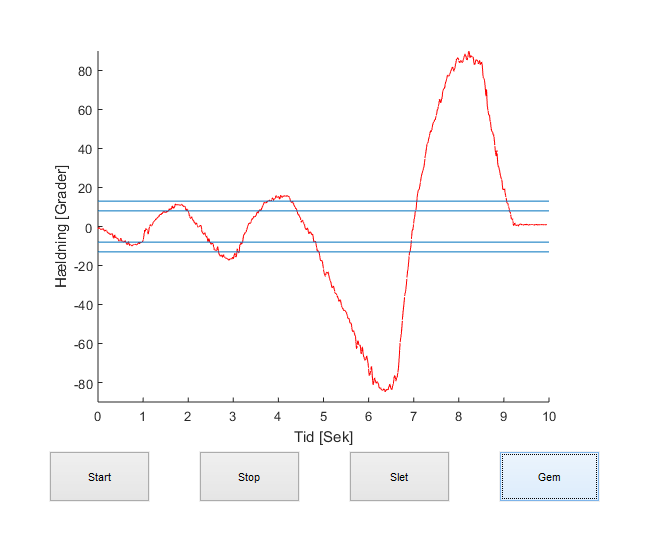
\includegraphics[scale=.6]{figures/cProblemloesning/Software.jpg}
	\caption{På figuren ses brugerfladen for programmet. De blå streger repræsenterer de definerede hældningsgrader, hvor der gives feedback i den analoge del. Den røde graf repræsenterer en måling foretaget med accelerometret. På x-aksen ses tiden og på y-aksen ses hældningsgrader af accelerometret.}
	\label{fig:samlet_system_digital}
\end{figure}
\noindent Det fremgår af \figref{fig:samlet_system_digital}, at signalet er kantet muligvis grundet støj. Derudover ses det, at den målte hældning af accelerometret kan aflæses på grafen, og denne kan gemmes vha. gemmefunktionen jævnfør afsnit \ref{software_test_implem}, side \pageref{software_test_implem}.\\
På baggrund af testen og \figref{fig:samlet_system_digital}  godkendes den digitale del af systemet og det vurderes, at det virker efter hensigten.